% This work is made available under the terms of the
% Creative Commons Attribution-ShareAlike 4.0 license,
% http://creativecommons.org/licenses/by-sa/4.0/.

\documentclass[a4paper]{book}

\usepackage{wrapfig}
\usepackage{graphicx}
\usepackage{hyperref}
\usepackage{multirow}
\usepackage{scalefnt}
\usepackage{tikz}

% watermark -- for draft stage
%\usepackage[firstpage]{draftwatermark}
%\SetWatermarkLightness{0.9}
%\SetWatermarkScale{5}

% This work is made available under the terms of the
% Creative Commons Attribution-ShareAlike 4.0 license,
% http://creativecommons.org/licenses/by-sa/4.0/.
%
% Version: $Revision: 2916 $

\newenvironment{tight_itemize}{
\begin{itemize}
  \setlength{\itemsep}{1pt}
  \setlength{\parskip}{0pt}
  \setlength{\parsep}{0pt}}{\end{itemize}
}

\newenvironment{tight_enumerate}{
\begin{enumerate}
  \setlength{\itemsep}{1pt}
  \setlength{\parskip}{0pt}
  \setlength{\parsep}{0pt}}{\end{enumerate}
}

% if you just need a simple heading
% Usage:
%   \heading{the text of the heading}
\newcommand{\heading}[1]{
  \vspace{0.3cm} \noindent \textbf{#1} \newline
}

\newcommand{\icon}[1]{\tikz[baseline=-3pt]\node[inner sep=0pt,outer sep=0pt]{\includegraphics[height=1.1em]{#1}};}


\title{
  \textbf{ADAMS} \\
  {\Large \textbf{A}dvanced \textbf{D}ata mining \textbf{A}nd \textbf{M}achine
  learning \textbf{S}ystem} \\
  {\Large Module: adams-security} \\
  \vspace{1cm}
  \includegraphics[width=4cm]{images/security-module.png} \\
}
\author{
  Peter Reutemann
}

\setcounter{secnumdepth}{3}
\setcounter{tocdepth}{3}

\begin{document}

\begin{titlepage}
\maketitle

\thispagestyle{empty}
\center
\begin{table}[b]
	\begin{tabular}{c l l}
		\parbox[c][2cm]{2cm}{\copyright 2019-2024} &
		\parbox[c][2cm]{5cm}{
\includegraphics[width=5cm]{images/coat_of_arms.pdf}} \\
	\end{tabular}
	
\includegraphics[width=12cm]{images/cc.png} \\
\end{table}

\end{titlepage}

\tableofcontents
\listoffigures
%\listoftables

%%%%%%%%%%%%%%%%%%%%%%%%%%%%%%%%%%%
\chapter{Introduction}
The \textit{adams-security} modules offers some rudimentary support around
generating, reading and writing key pairs. It also allows you to configure
an SSL (or TLS) context.

For inspecting keystore files or similar, you might want to look at the
cross-platform Keystore Explorer\cite{kse} tool.

%%%%%%%%%%%%%%%%%%%%%%%%%%%%%%%%%%%
\chapter{Flow}
\noindent The following standalone actors are available:
\begin{tight_itemize}
  \item \textit{KeyManager} - for configuring a KeyManagerFactory instance.
  \item \textit{TrustManager} - for configuring a TrustManagerFactory instance.
  \item \textit{SSLContext} - for setting up an SSL context.
\end{tight_itemize}

\noindent The following sources are available:
\begin{tight_itemize}
  \item \textit{KeyPairFileReader} - for reading private/public key pair in
  DER format from disk.
  \item \textit{KeyPairGenerator} - for generating key pairs (e.g., RSA).
\end{tight_itemize}

\noindent The following transformers are available:
\begin{tight_itemize}
  \item \textit{GetKeyFromKeyPair} - retrieves private or public key from pair.
\end{tight_itemize}

\noindent The following sinks are available:
\begin{tight_itemize}
  \item \textit{KeyPairFileWriter} - for writing key pairs to disk (in DER format).
\end{tight_itemize}

\noindent The following control actors are available:
\begin{tight_itemize}
  \item \textit{Keytool} - for executing the \verb|keytool| executable, forwards
  the generated output to its sub-actors.
\end{tight_itemize}


%%%%%%%%%%%%%%%
% Preferences %
%%%%%%%%%%%%%%%
\chapter{Preferences}
In the \textit{Trust store} section of the global preferences of ADAMS (in the main menu,
select *Program* and then *Preferences*), you can specify a Java trust store to use
globally (see figure \ref{preferences_truststore}). This can be used, e.g., for connecting
to MySQL databases that require SSL connections.
\begin{figure}[htb]
  \centering
  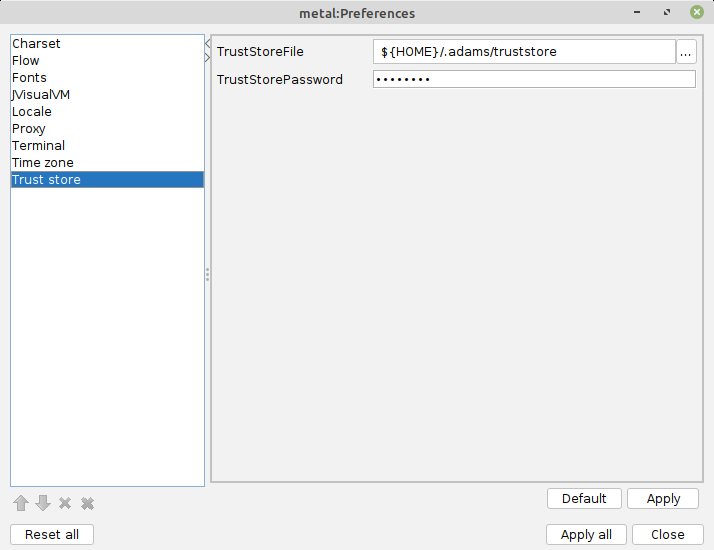
\includegraphics[width=12.0cm]{images/preferences_truststore.png}
  \caption{Preferences for specifying trust store}
  \label{preferences_truststore}
\end{figure}


%%%%%%%%%%%%%%%%%%%%%%%%%%%%%%%%%%%
% This work is made available under the terms of the 
% Creative Commons Attribution-ShareAlike 4.0 license,
% http://creativecommons.org/licenses/by-sa/4.0/.

\begin{thebibliography}{999}
	% to make the bibliography appear in the TOC
	\addcontentsline{toc}{chapter}{Bibliography}

    % references
	\bibitem{adams}
		\textit{ADAMS} -- Advanced Data mining and Machine learning System \\
		\url{https://adams.cms.waikato.ac.nz/}{}

	\bibitem{djl}
		\textit{Deep Java Library} -- open source library to build and deploy deep learning in Java. \\
		\url{https://djl.ai/}{}

\end{thebibliography}


\end{document}
